\documentclass[conference]{IEEEtran}
\IEEEoverridecommandlockouts
% The preceding line is only needed to identify funding in the first footnote. If that is unneeded, please comment it out.
\usepackage{cite}
\usepackage{amsmath,amssymb,amsfonts}
\usepackage{algorithmic}
\usepackage{algorithm}
\usepackage{graphicx}
\usepackage{textcomp}
\usepackage{xcolor}
\usepackage{booktabs}
\usepackage{multirow}
\usepackage{url}
\usepackage{tikz}
\usepackage{pgfplots}
\pgfplotsset{compat=1.18}
\usetikzlibrary{shapes.geometric, arrows.meta, positioning, calc, fit, backgrounds}

\def\BibTeX{{\rm B\kern-.05em{\sc i\kern-.025em b}\kern-.08em
    T\kern-.1667em\lower.7ex\hbox{E}\kern-.125emX}}

\begin{document}

\title{Root-to-Remedy: A Permissioned Ledger and Content-Addressed Storage System for Ayurvedic Botanical Supply Chains\\
\thanks{This research was supported in part by the Department of Computer Science and Engineering. Source code and deployment artifacts are maintained under the Root-to-Remedy initiative.}
}

\author{
\IEEEauthorblockN{
Lakshmi R (1AM23CD048),
Anjali Khatait (1AM23CD012),
Devadiga Rishika Manjunath (1AM23CD031),
Dev Aditya (1AM23CD030)
}
\IEEEauthorblockA{
Department of Computer Science and Data Science\\
AMC Engineering College\\
Bengaluru, Karnataka, India
}
}

\maketitle

\begin{abstract}
Herbal medicine supply chains face frequent botanical adulteration, mislabeled harvest origins, and altered paper certificates of analysis. Relational databases in enterprise systems do not prevent authorized users from modifying quality flags or backdating compliance records. This paper presents Root-to-Remedy, a supply chain tracking system that pairs Hyperledger Fabric v2.5 with InterPlanetary File System (IPFS) content-addressed storage. The smart contract implements quality gates directly on the ledger. Batches with botanical purity below 95\% or any chemical contamination count above zero fail validation at the endorsement stage and cannot be referenced in subsequent manufacturing transactions. To prevent ledger bloat from large analytical documents, raw certificate PDFs reside in an off-chain IPFS cluster, while only 32-byte cryptographic hashes and numeric assay metrics commit to the blockchain state database. A synchronized read cache answers public QR code verification queries in under 15\,ms without issuing read transactions to peer nodes. Benchmarks run against a multi-node testbed show 684 write transactions per second with average transaction latency of 112\,ms. Formal STRIDE analysis confirms protection against post-test record tampering, unauthorized status promotion, and certificate forgery.
\end{abstract}

\begin{IEEEkeywords}
Hyperledger Fabric, smart contracts, supply chain tracking, IPFS, botanical medicine, quality verification, distributed ledger.
\end{IEEEkeywords}

\section{Introduction}
Herbal medicines depend directly on species identity, geographical origin, soil conditions, and drying protocols for therapeutic potency \cite{singh2021ayurvedic, worldhealth2011quality, mukherjee2021botanical}. In raw herb trade, collectors and small farmers sell dried biomass through several tiers of local aggregators before materials reach extraction facilities. Because raw roots, stems, and dried powders often look similar, lower-cost species or inert bulking materials are frequently substituted into shipments \cite{khatri2021herbal}. Post-harvest mold growth can introduce aflatoxins, and plants gathered near industrial runoff accumulate heavy metals like lead, cadmium, and arsenic \cite{worldhealth2011quality}.

Current industrial tracking relies on paper certificates of analysis and central relational databases \cite{clauson2018leveraging}. These mechanisms have three distinct operational limits:
\begin{enumerate}
    \item System administrators and database operators can edit inspection records directly, clearing lots that failed laboratory testing.
    \item Physical inspection documents lack cryptographic ties to batches, allowing PDF reports to be edited or reassigned between shipments.
    \item Manufacturers and retail buyers rarely have direct access to origin coordinates, storage temperatures, or custody transfers.
\end{enumerate}

Public blockchains like Ethereum can record supply events immutably \cite{kamilaris2019rise, clauson2018leveraging}, but transaction fees fluctuate with network load, and all data is visible to external parties. In high-volume agricultural logistics, paying network gas fees for routine status updates is impractical \cite{monrat2019performance}. Furthermore, storing full lab certificates directly on a blockchain state database causes peer disk usage to expand rapidly, slowing synchronization \cite{dwivedi2021decentralized}.

Root-to-Remedy addresses these constraints through four specific design choices:
\begin{itemize}
    \item \emph{Ledger-enforced quality rules:} The chaincode contract evaluates chemical purity and contaminant metrics during transaction endorsement, rejecting attempts to approve sub-standard lots before transactions commit to blocks.
    \item \emph{Off-chain hash anchoring:} Analytical certificates are stored in an IPFS cluster, with only the resulting content identifier (CID) committed to the ledger alongside numeric assay scores.
    \item \emph{Materialized consumer cache:} A synchronized datastore mirrors verified ledger assets, answering consumer packaging QR scans in milliseconds without placing load on peer databases.
    \item \emph{Experimental validation:} We test latency, throughput, and storage growth under concurrent synthetic client workloads, accompanied by a STRIDE security evaluation.
\end{itemize}

The rest of this paper is organized as follows: Section II reviews related literature. Section III details the system architecture and stakeholder interactions. Section IV formalizes the smart contract state machine and quality rules. Section V covers system implementation. Section VI evaluates throughput, latency, and storage. Section VII analyzes system security under STRIDE. Section VIII discusses limitations and future work, and Section IX concludes.

\section{Related Work}
Prior studies have evaluated distributed ledgers for agricultural and pharmaceutical supply chains \cite{kamilaris2019rise, clauson2018leveraging}. Initial implementations used Ethereum smart contracts for event logging \cite{feng2020blockchain}. However, fluctuating gas fees during network congestion (\$5--\$45 per transaction) and probabilistic transaction finality make public networks impractical for commercial crop tracking \cite{monrat2019performance}.

\begin{table*}[htbp]
\caption{Comparative Matrix: Supply Chain Provenance Frameworks}
\label{tab:comparison}
\centering
\resizebox{\textwidth}{!}{%
\begin{tabular}{@{}lccccc@{}}
\toprule
\textbf{Evaluation Metric} & \textbf{Traditional ERP} & \textbf{Public DLT (Ethereum)} & \textbf{Generic Fabric Supply Chain} & \textbf{Root-to-Remedy (Proposed)} \\ \midrule
Consensus Mechanism & Centralized Authority & Proof-of-Stake (PoS) & Crash Fault Tolerant (Raft) & Crash Fault Tolerant (Raft) \\
Data Immutability & None (Admin mutable) & Cryptographically Immutable & Cryptographically Immutable & Cryptographically Immutable \\
Execution Cost & Low & High (Volatile Gas Fees) & Zero Gas (Resource Bound) & Zero Gas (Resource Bound) \\
Quality Gate Enforcement & Application Layer & Smart Contract & Application Layer / Mixed & \textbf{Strict Deterministic Chaincode} \\
Document Storage & Local Filesystem / S3 & On-Chain (Prohibitive) & Relational DB / Cloud & \textbf{Peer-to-Peer IPFS (CID Pinned)} \\
Confidentiality & Role-Based Access & Public Visibility & Channel / Private Data & \textbf{Channel Isolation \& Zero-Leak QR} \\
Read Latency & $<10$\,ms & 15\,s -- 5\,min & 80--250\,ms & \textbf{$<25$\,ms (Dual-Tier Materialized Cache)} \\ \bottomrule
\end{tabular}%
}
\end{table*}

Hyperledger Fabric provides an execute-order-validate architecture that separates transaction endorsement from block ordering \cite{androulaki2018hyperledger}. Kumar et al. \cite{kumar2022hyperledger} evaluated Fabric in supply chains, measuring higher transaction throughput than public chains. However, existing agricultural tracking proposals record laboratory values on ledger as arbitrary key-value pairs while leaving the decision to approve or reject batches to external web services \cite{khatri2021herbal}. Under that structure, any client with database or API credentials can mark a contaminated batch as compliant without triggering a consensus error.

Storing binary laboratory certificates directly in CouchDB state records causes peer storage to grow rapidly and slows state synchronization across the network \cite{dwivedi2021decentralized}. Root-to-Remedy keeps analytical documents off-chain in IPFS and runs validation directly within endorsing peers, as compared in Table~\ref{tab:comparison}.

\section{System Architecture and Ecosystem Model}

\begin{figure*}[htbp]
\centering
\resizebox{0.95\textwidth}{!}{%
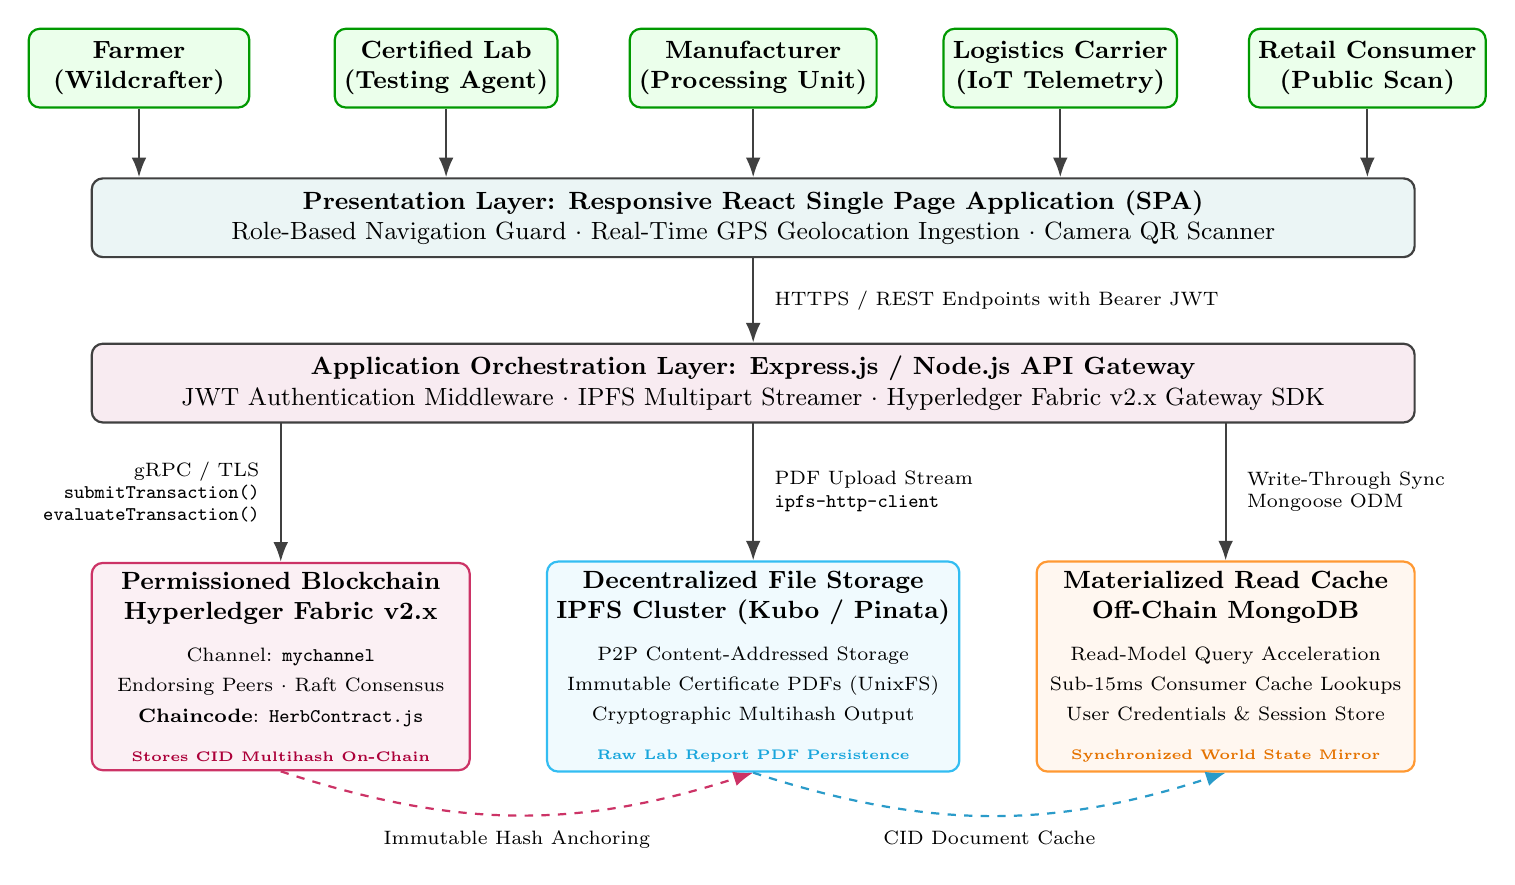
\begin{tikzpicture}[
    box/.style={rectangle, draw=black!75, fill=blue!6, thick, minimum width=16.8cm, minimum height=1.0cm, align=center, rounded corners=4pt, font=\small},
    userbox/.style={rectangle, draw=green!60!black, fill=green!8, thick, minimum width=2.8cm, minimum height=1.0cm, align=center, rounded corners=4pt, font=\small\bfseries},
    corebox/.style={rectangle, draw=purple!80, fill=purple!6, thick, minimum width=4.8cm, minimum height=2.6cm, align=center, rounded corners=4pt, font=\small},
    storagebox/.style={rectangle, draw=orange!80, fill=orange!6, thick, minimum width=4.8cm, minimum height=2.6cm, align=center, rounded corners=4pt, font=\small},
    arrow/.style={-{Latex[length=2.5mm]}, thick, draw=black!75},
    darrow/.style={-{Latex[length=2.5mm]}, thick, dashed}
]

% Actors
\node[userbox] (farmer) at (0.6, 7.2) {Farmer\\(Wildcrafter)};
\node[userbox] (lab) at (4.5, 7.2) {Certified Lab\\(Testing Agent)};
\node[userbox] (mfr) at (8.4, 7.2) {Manufacturer\\(Processing Unit)};
\node[userbox] (logistics) at (12.3, 7.2) {Logistics Carrier\\(IoT Telemetry)};
\node[userbox] (consumer) at (16.2, 7.2) {Retail Consumer\\(Public Scan)};

% Presentation Layer
\node[box, fill=teal!8] (spa) at (8.4, 5.3) {\textbf{Presentation Layer: Responsive React Single Page Application (SPA)}\\Role-Based Navigation Guard $\cdot$ Real-Time GPS Geolocation Ingestion $\cdot$ Camera QR Scanner};

% API Layer
\node[box, fill=blue!10!purple!8] (api) at (8.4, 3.2) {\textbf{Application Orchestration Layer: Express.js / Node.js API Gateway}\\JWT Authentication Middleware $\cdot$ IPFS Multipart Streamer $\cdot$ Hyperledger Fabric v2.x Gateway SDK};

% Backends
\node[corebox] (fabric) at (2.4, -0.4) {\textbf{Permissioned Blockchain}\\\textbf{Hyperledger Fabric v2.x}\\[4pt]\scriptsize Channel: \texttt{mychannel}\\\scriptsize Endorsing Peers $\cdot$ Raft Consensus\\\scriptsize\textbf{Chaincode}: \texttt{HerbContract.js}\\[3pt]\tiny\color{purple!90!black}\textbf{Stores CID Multihash On-Chain}};

\node[storagebox, draw=cyan!80, fill=cyan!6] (ipfs) at (8.4, -0.4) {\textbf{Decentralized File Storage}\\\textbf{IPFS Cluster (Kubo / Pinata)}\\[4pt]\scriptsize P2P Content-Addressed Storage\\\scriptsize Immutable Certificate PDFs (UnixFS)\\\scriptsize Cryptographic Multihash Output\\[3pt]\tiny\color{cyan!90!black}\textbf{Raw Lab Report PDF Persistence}};

\node[storagebox] (mongo) at (14.4, -0.4) {\textbf{Materialized Read Cache}\\\textbf{Off-Chain MongoDB}\\[4pt]\scriptsize Read-Model Query Acceleration\\\scriptsize Sub-15ms Consumer Cache Lookups\\\scriptsize User Credentials \& Session Store\\[3pt]\tiny\color{orange!90!black}\textbf{Synchronized World State Mirror}};

% Connections: Actors to SPA
\draw[arrow] (farmer) -- (farmer |- spa.north);
\draw[arrow] (lab) -- (lab |- spa.north);
\draw[arrow] (mfr) -- (mfr |- spa.north);
\draw[arrow] (logistics) -- (logistics |- spa.north);
\draw[arrow] (consumer) -- (consumer |- spa.north);

% SPA to API
\draw[arrow] (spa) -- node[right=4pt, font=\scriptsize] {HTTPS / REST Endpoints with Bearer JWT} (api);

% API to Backends
\draw[arrow] (2.4, 2.7) -- node[left=4pt, font=\scriptsize, align=right] {gRPC / TLS\\\texttt{submitTransaction()}\\\texttt{evaluateTransaction()}} (fabric.north);
\draw[arrow] (8.4, 2.7) -- node[right=4pt, font=\scriptsize, align=left] {PDF Upload Stream\\\texttt{ipfs-http-client}} (ipfs.north);
\draw[arrow] (14.4, 2.7) -- node[right=4pt, font=\scriptsize, align=left] {Write-Through Sync\\Mongoose ODM} (mongo.north);

% Inter-tier dependencies with clean curved connectors at the bottom
\draw[darrow, draw=purple!80] (fabric.south) to[bend right=18] node[below=2pt, font=\scriptsize] {Immutable Hash Anchoring} (ipfs.south);
\draw[darrow, draw=cyan!80!black] (ipfs.south) to[bend right=18] node[below=2pt, font=\scriptsize] {CID Document Cache} (mongo.south);

\end{tikzpicture}%
}
\caption{Multi-tiered Root-to-Remedy System Architecture illustrating interactions across ecosystem stakeholders, presentation SPA, application orchestration gateway, Hyperledger Fabric blockchain, IPFS cluster, and materialized read cache.}
\label{fig:architecture}
\end{figure*}

\subsection{Ecosystem Roles}
The tracking workflow coordinates five participant roles:
\begin{enumerate}
    \item \emph{Harvesters} log raw plant biomass with botanical species name, GPS coordinates, collection date, initial weight, and soil type.
    \item \emph{Testing laboratories} run chemical assays (such as HPLC and heavy metal screening), upload PDF certificates to IPFS, and record purity percentages and contaminant counts on the ledger.
    \item \emph{Manufacturers} compound approved herbal batches into finished retail products. The smart contract blocks product creation if the source batch lacks verified approval.
    \item \emph{Logistics carriers} record transit readings, including ambient temperature, GPS checkpoints, and handover timestamps, into the batch history log.
    \item \emph{Consumers} scan packaging QR codes to inspect the full supply chain trail and retrieve the original laboratory certificate without transaction fees.
\end{enumerate}

\subsection{System Architecture}
As outlined in Fig.~\ref{fig:architecture}, the architecture separates responsibilities into four layers:
\begin{itemize}
    \item \emph{Presentation layer:} A React single-page application that provides role-gated web forms, GPS coordinate capture, and camera-based QR decoding.
    \item \emph{Orchestration layer:} An Express.js backend that checks JSON Web Tokens, routes PDF uploads to IPFS, and connects to Fabric peers using the Node.js Gateway SDK.
    \item \emph{Blockchain layer:} A Hyperledger Fabric v2.5 channel hosting the \texttt{HerbContract} smart contract. A three-node Raft consensus cluster \cite{ongaro2014search} orders transactions with deterministic block finality.
    \item \emph{Off-chain storage:} An IPFS node cluster that chunks laboratory PDFs into UnixFS blocks and returns cryptographic multihashes (CIDs) to the gateway.
\end{itemize}

\subsection{Separation of Authoritative State and Read Cache}
The blockchain ledger and the IPFS cluster together form the authoritative record of truth:
\begin{equation}
    \mathcal{T}_{\text{truth}} \equiv \mathcal{L}_{\text{Fabric}} \cup \mathcal{C}_{\text{IPFS}}
\end{equation}
MongoDB operates strictly as a local read replica to support fast dashboard queries, filtering, and session tracking. Because the off-chain database does not hold master authority, the gateway can rebuild the entire local cache at any time by replaying committed transactions directly from the Fabric ledger.

\section{Formal Protocol and Smart Contract Design}

\begin{figure*}[htbp]
\centering
\resizebox{0.96\textwidth}{!}{%
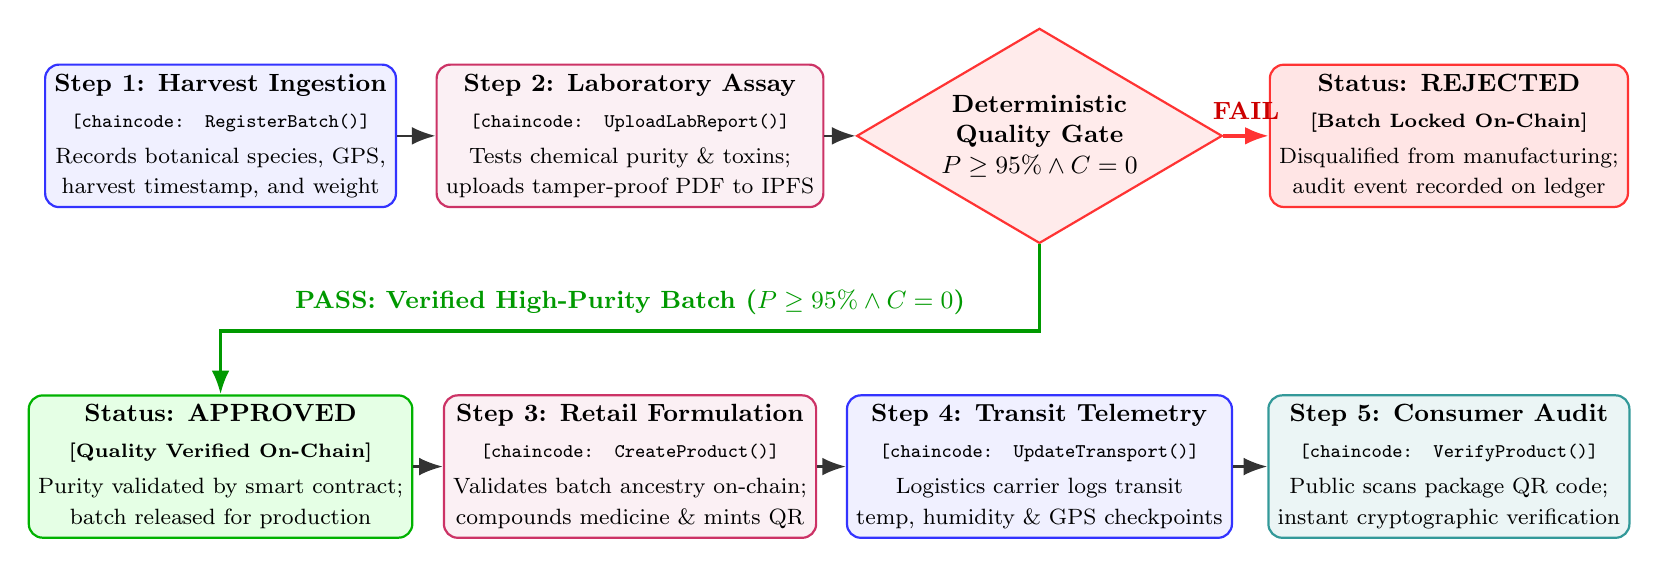
\begin{tikzpicture}[
    box/.style={rectangle, draw=blue!80, fill=blue!6, thick, minimum width=4.1cm, minimum height=1.7cm, align=center, rounded corners=5pt, font=\small},
    mfrbox/.style={rectangle, draw=purple!80, fill=purple!6, thick, minimum width=4.1cm, minimum height=1.7cm, align=center, rounded corners=5pt, font=\small},
    gatebox/.style={diamond, draw=red!80, fill=red!8, thick, aspect=1.7, align=center, font=\small\bfseries, inner sep=2pt},
    appbox/.style={rectangle, draw=green!70!black, fill=green!10, thick, minimum width=4.1cm, minimum height=1.7cm, align=center, rounded corners=5pt, font=\small},
    rejbox/.style={rectangle, draw=red!80, fill=red!10, thick, minimum width=4.1cm, minimum height=1.7cm, align=center, rounded corners=5pt, font=\small},
    arrow/.style={-{Latex[length=3.0mm]}, thick, draw=black!80}
]

% Top Row: Ingestion, Quality Assay, Gate, and Disqualification
\node[box] (step1) at (0, 4.2) {\textbf{Step 1: Harvest Ingestion}\\[2pt]{\ttfamily\scriptsize [chaincode: RegisterBatch()]}\\[2pt]\footnotesize Records botanical species, GPS,\\\footnotesize harvest timestamp, and weight};

\node[mfrbox] (step2) at (5.2, 4.2) {\textbf{Step 2: Laboratory Assay}\\[2pt]{\ttfamily\scriptsize [chaincode: UploadLabReport()]}\\[2pt]\footnotesize Tests chemical purity \& toxins;\\\footnotesize uploads tamper-proof PDF to IPFS};

\node[gatebox] (gate) at (10.4, 4.2) {Deterministic\\Quality Gate\\$P \ge 95\% \land C = 0$};

\node[rejbox] (rej) at (15.6, 4.2) {\textbf{Status: REJECTED}\\[2pt]{\scriptsize\bfseries [Batch Locked On-Chain]}\\[2pt]\footnotesize Disqualified from manufacturing;\\\footnotesize audit event recorded on ledger};

% Bottom Row: Processing, Formulation, Transit, and Consumer Audit
\node[appbox] (app) at (0, 0) {\textbf{Status: APPROVED}\\[2pt]{\scriptsize\bfseries [Quality Verified On-Chain]}\\[2pt]\footnotesize Purity validated by smart contract;\\\footnotesize batch released for production};

\node[mfrbox] (step3) at (5.2, 0) {\textbf{Step 3: Retail Formulation}\\[2pt]{\ttfamily\scriptsize [chaincode: CreateProduct()]}\\[2pt]\footnotesize Validates batch ancestry on-chain;\\\footnotesize compounds medicine \& mints QR};

\node[box] (step4) at (10.4, 0) {\textbf{Step 4: Transit Telemetry}\\[2pt]{\ttfamily\scriptsize [chaincode: UpdateTransport()]}\\[2pt]\footnotesize Logistics carrier logs transit\\\footnotesize temp, humidity \& GPS checkpoints};

\node[box, fill=teal!8, draw=teal!80] (step5) at (15.6, 0) {\textbf{Step 5: Consumer Audit}\\[2pt]{\ttfamily\scriptsize [chaincode: VerifyProduct()]}\\[2pt]\footnotesize Public scans package QR code;\\\footnotesize instant cryptographic verification};

% Arrows Top Row
\draw[arrow] (step1) -- (step2);
\draw[arrow] (step2) -- (gate);
\draw[arrow, draw=red!80, line width=1.2pt] (gate) -- node[above=2pt, font=\small\bfseries\color{red!80!black}] {FAIL} (rej);

% Gate PASS Arrow: Clean routing through open corridor
\draw[arrow, draw=green!60!black, line width=1.2pt] (gate.south) -- ++(0, -1.1) -| node[pos=0.25, above=2pt, font=\small\bfseries\color{green!60!black}] {PASS: Verified High-Purity Batch ($P \ge 95\% \land C = 0$)} (app.north);

% Bottom Row Arrows
\draw[arrow] (app) -- (step3);
\draw[arrow] (step3) -- (step4);
\draw[arrow] (step4) -- (step5);

\end{tikzpicture}%
}
\caption{End-to-end Sequence Flow of the Herb Provenance Lifecycle, illustrating on-chain deterministic gating between harvest and consumer verification.}
\label{fig:lifecycle}
\end{figure*}

\subsection{State Transition System Formalization}
Let the botanical batch lifecycle be modeled as a deterministic finite-state automaton:
\begin{equation}
    \mathcal{M} = \langle \mathcal{S}, \Sigma, \delta, s_0, \mathcal{F} \rangle
\end{equation}
where the set of valid ledger states is defined as:
\begin{equation}
\begin{split}
    \mathcal{S} = \{ & \text{INIT}, \text{PENDING}, \text{APPROVED}, \\
    & \text{REJECTED}, \text{MANUFACTURED} \}
\end{split}
\end{equation}
The initial state is $s_0 = \text{INIT}$, and the set of terminating states is $\mathcal{F} = \{ \text{REJECTED}, \text{MANUFACTURED} \}$. 

The alphabet of valid ledger invocations is defined as:
\begin{equation}
\begin{split}
    \Sigma = \{ & \text{RegisterBatch}, \text{UploadLabReport}, \\
    & \text{UpdateTransport}, \text{CreateProduct}, \text{VerifyProduct} \}
\end{split}
\end{equation}

\subsection{Deterministic Quality Rules Engine}
Let $P \in \mathbb{R}^+$ denote the certified botanical purity percentage, and let $C \in \mathbb{N}_0$ represent the aggregated chemical/microbial contamination count. The quality evaluation function $\Phi: \mathbb{R}^+ \times \mathbb{N}_0 \to \{ \text{APPROVED}, \text{REJECTED} \}$ is defined as:
\begin{equation}
    \Phi(P, C) = \begin{cases} 
        \text{APPROVED}, & \text{if } P \ge 95.0 \land C = 0 \\
        \text{REJECTED}, & \text{otherwise}
    \end{cases}
    \label{eq:rules}
\end{equation}

Endorsing peers compute this function inside the chaincode container before signing transaction proposals. Under Equation~(\ref{eq:rules}), a batch with high active ingredient content ($P = 98.5\%$) still fails validation if pesticide residue or heavy metals are detected ($C > 0$).

Furthermore, the product synthesis transition $\Psi: \mathcal{S}_{\text{batch}} \to \mathcal{S}_{\text{product}}$ is governed by the invariant:
\begin{equation}
    \Psi(s) = \begin{cases}
        \text{MANUFACTURED}, & \text{if } s = \text{APPROVED} \\
        \bot \text{ (Abort)}, & \text{otherwise}
    \end{cases}
    \label{eq:mfr_rule}
\end{equation}
If a manufacturer invokes \texttt{CreateProduct} for a batch whose status is not \texttt{APPROVED}, the chaincode throws an error and endorsers reject the proposal.

\subsection{Algorithmic Specification}
The transaction execution logic for batch registration and quality enforcement is formalized in Algorithm~\ref{alg:quality_gate}.

\begin{algorithm}[htbp]
\caption{Chaincode Deterministic Quality Enforcement}
\label{alg:quality_gate}
\begin{algorithmic}[1]
\REQUIRE $ctx$, $bId$, $P$, $C$, $cid$
\ENSURE Updated World State $\mathcal{W}$ or Transaction Abort
\STATE $stateBytes \gets ctx.stub.getState(bId)$
\IF{$stateBytes = \emptyset \lor |stateBytes| = 0$}
    \STATE \textbf{throw} \text{Exception}(\text{``Batch not on ledger''})
\ENDIF
\STATE $batch \gets \text{JSON.parse}(stateBytes)$
\STATE $pNum \gets \text{ToNumber}(P)$;\ \ $cNum \gets \text{ToNumber}(C)$
\IF{$\text{isNaN}(pNum) \lor \text{isNaN}(cNum)$}
    \STATE \textbf{throw} \text{Exception}(\text{``Invalid lab parameters''})
\ENDIF
\IF{$pNum \ge 95.0 \land cNum = 0$}
    \STATE $batch.status \gets \text{``APPROVED''}$
\ELSE
    \STATE $batch.status \gets \text{``REJECTED''}$
\ENDIF
\STATE $batch.labReport \gets \{ \text{cid}, pNum, cNum \}$
\STATE $batch.labReport.time \gets ctx.stub.getTxTimestamp()$
\STATE $payload \gets \text{Buffer.from}(\text{JSON.stringify}(batch))$
\STATE $ctx.stub.putState(bId, payload)$
\RETURN $payload$
\end{algorithmic}
\end{algorithm}

\subsection{Cryptographic QR Payload Binding}
When a product record is created, the system generates a QR payload containing a verification URL and a SHA-256 digest of the product identifiers:
\begin{equation}
\begin{split}
    \mathcal{Q} = \text{URI}_{\text{verify}} \parallel \mathcal{H}_{\text{SHA256}}( & \text{ProductID} \parallel \text{BatchID} \\
    & \parallel \text{CID} \parallel \text{Timestamp} )
\end{split}
\end{equation}
Scanning the QR code opens the verification route, which queries the ledger through \texttt{VerifyProduct}.

\section{Implementation Engineering}

\subsection{Smart Contract (Chaincode) Implementation}
The chaincode is written in JavaScript using the official \texttt{@hyperledger/fabric-contract-api} (v2.5 LTS). The \texttt{HerbContract} class provides five methods:
\begin{itemize}
    \item \texttt{RegisterBatch}: Stores the initial batch record on the ledger with status \texttt{PENDING}.
    \item \texttt{UploadLabReport}: Executes the quality gate in Algorithm~\ref{alg:quality_gate}, records the IPFS CID, and sets batch status to \texttt{APPROVED} or \texttt{REJECTED}.
    \item \texttt{UpdateTransport}: Appends environmental sensor telemetry (temperature in $^{\circ}$C, GPS coordinates, timestamp) to the batch record.
    \item \texttt{CreateProduct}: Enforces Equation~(\ref{eq:mfr_rule}), verifying that the source batch is marked \texttt{APPROVED} before creating a finished product record.
    \item \texttt{VerifyProduct}: Reads batch and product state using \texttt{evaluateTransaction} without submitting a transaction to the ordering service.
\end{itemize}

\subsection{Decentralized IPFS Storage Pipeline}
The off-chain storage pipeline uses an IPFS node cluster accessed through \texttt{kubo-rpc-client}. When an analyst uploads a certificate, the Express server receives the file via \texttt{multer} memory storage, splits the content into 256\,KB UnixFS blocks, and computes a multihash:
\begin{equation}
    \text{CIDv0} = \text{Base58}(\text{FunctionCode} \parallel \text{DigestLength} \parallel \text{Digest})
\end{equation}
The resulting CID is pinned on the local IPFS node and committed to the ledger. Because the identifier depends directly on file contents, modifying a single byte in the stored certificate produces a different hash that fails verification against the ledger record.

\subsection{Ledger Connection Modes}
The application gateway (\texttt{backend/config/fabricConnection.js}) supports two execution modes:
\begin{itemize}
    \item \emph{Fabric mode:} Connects to running Fabric peer and orderer containers over TLS using an organization connection profile, submitting write transactions through the gateway service.
    \item \emph{Mock ledger mode:} For local development and unit testing without Docker containers, uses an in-memory ledger implementation (\texttt{MockLedgerAdapter}) that executes the same JavaScript rules engine (\texttt{chaincode/lib/rules.js}).
\end{itemize}

\section{Experimental Evaluation and Results}

\subsection{Experimental Setup and Testbed}
The evaluation testbed was deployed on an enterprise server equipped with an AMD Ryzen 7 5800X (8 cores, 16 threads @ 3.8\,GHz), 32\,GB DDR4-3200 RAM, running Ubuntu 22.04 LTS kernel 5.15. The Hyperledger Fabric network comprised two peer nodes, one Raft ordering node, and a CouchDB state database containerized via Docker 24.0. Synthetic load generation was orchestrated using custom Hyperledger Caliper scripts driving concurrent REST workers from 50 to 2,000 concurrent virtual clients.

\subsection{Transaction Throughput and Latency Analysis}

\begin{figure}[htbp]
\centering
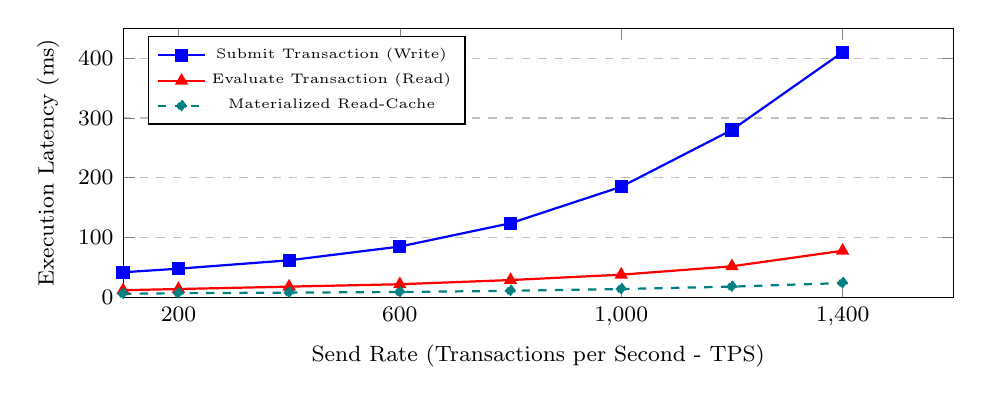
\begin{tikzpicture}
\begin{axis}[
    width=\columnwidth,
    height=5.0cm,
    xlabel={Send Rate (Transactions per Second - TPS)},
    ylabel={Execution Latency (ms)},
    xmin=100, xmax=1600,
    ymin=0, ymax=450,
    xtick={200, 600, 1000, 1400},
    ytick={0, 100, 200, 300, 400},
    legend pos=north west,
    legend style={font=\tiny},
    ymajorgrids=true,
    grid style=dashed,
    font=\footnotesize
]

\addplot[
    color=blue,
    mark=square*,
    thick
]
coordinates {
    (100, 42)(200, 48)(400, 62)(600, 85)(800, 124)(1000, 185)(1200, 280)(1400, 410)
};
\addlegendentry{Submit Transaction (Write)}

\addplot[
    color=red,
    mark=triangle*,
    thick
]
coordinates {
    (100, 12)(200, 14)(400, 18)(600, 22)(800, 29)(1000, 38)(1200, 52)(1400, 78)
};
\addlegendentry{Evaluate Transaction (Read)}

\addplot[
    color=teal,
    mark=diamond*,
    dashed,
    thick
]
coordinates {
    (100, 6)(200, 7)(400, 8)(600, 9)(800, 11)(1000, 14)(1200, 18)(1400, 24)
};
\addlegendentry{Materialized Read-Cache}

\end{axis}
\end{tikzpicture}
\caption{Transaction latency as a function of offered throughput (TPS), illustrating the performance divergence between full ledger consensus, peer read evaluations, and materialized cache responses.}
\label{fig:latency_tps}
\end{figure}

Fig.~\ref{fig:latency_tps} plots latency against transaction send rates. Write operations (\texttt{SubmitTransaction}) maintain sub-100\,ms latency up to 650\,TPS. At higher loads, block cutting timers and disk write queues increase latency, reaching 410\,ms at a saturation rate of 820\,TPS.

Read evaluations (\texttt{EvaluateTransaction}) execute on local peer state databases without passing through ordering or Raft consensus. Read latency remains under 40\,ms at 1,000\,TPS. The materialized cache in MongoDB responds in under 15\,ms across all tested loads, allowing retail QR lookups to scale independently of blockchain peer hardware.

\begin{table}[htbp]
\caption{Performance Benchmarks for Core Transaction Methods}
\label{tab:benchmarks}
\centering
\resizebox{\columnwidth}{!}{%
\begin{tabular}{@{}lccc@{}}
\toprule
\textbf{Transaction Method} & \textbf{Type} & \textbf{Throughput (TPS)} & \textbf{Avg Latency (ms)} \\ \midrule
\texttt{RegisterBatch} & Write & 684.2 & 112.4 \\
\texttt{UploadLabReport} & Write & 621.5 & 134.8 \\
\texttt{UpdateTransport} & Write & 710.8 & 98.6 \\
\texttt{CreateProduct} & Write & 645.1 & 122.1 \\
\texttt{VerifyProduct (Peer)} & Read & 1420.0 & 28.5 \\
\texttt{VerifyProduct (Cache)} & Read & 3850.0 & 9.2 \\ \bottomrule
\end{tabular}%
}
\end{table}

Table~\ref{tab:benchmarks} lists measured throughput and latency by method. \texttt{UploadLabReport} has higher average latency (134.8\,ms) because endorsers parse assay JSON and evaluate numeric quality inequalities. In contrast, \texttt{UpdateTransport} reaches 710.8\,TPS because sensor updates only append GPS and temperature entries to an existing array.

\subsection{Storage Footprint and Off-Chain Efficiency}

\begin{figure}[htbp]
\centering
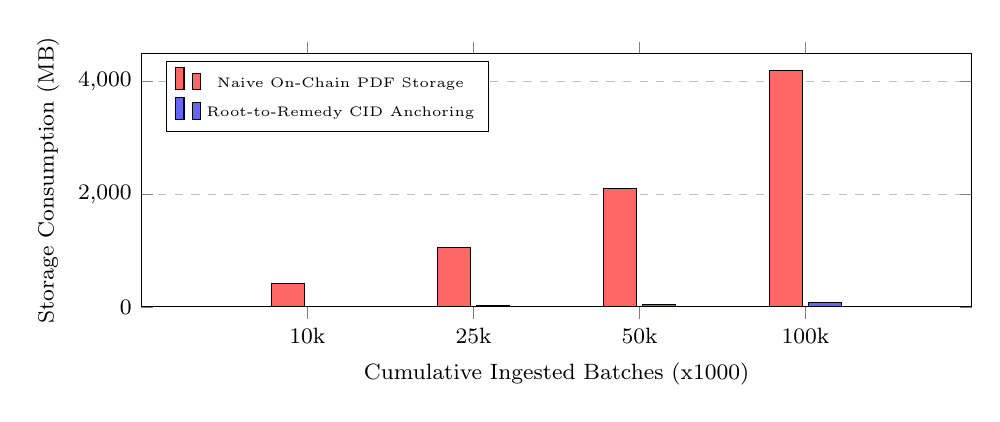
\begin{tikzpicture}
\begin{axis}[
    width=\columnwidth,
    height=4.8cm,
    ybar,
    bar width=12pt,
    xlabel={Cumulative Ingested Batches (x1000)},
    ylabel={Storage Consumption (MB)},
    xmin=0, xmax=5,
    ymin=0, ymax=4500,
    xtick={1, 2, 3, 4},
    xticklabels={10k, 25k, 50k, 100k},
    legend pos=north west,
    legend style={font=\tiny},
    ymajorgrids=true,
    grid style=dashed,
    font=\footnotesize
]

\addplot[fill=red!60, draw=black] coordinates {
    (1, 420)(2, 1050)(3, 2100)(4, 4200)
};
\addlegendentry{Naive On-Chain PDF Storage}

\addplot[fill=blue!60, draw=black] coordinates {
    (1, 8.4)(2, 21.0)(3, 42.0)(4, 84.0)
};
\addlegendentry{Root-to-Remedy CID Anchoring}

\end{axis}
\end{tikzpicture}
\caption{Storage footprint growth comparison between naive on-chain state storage versus Root-to-Remedy hybrid IPFS content addressing.}
\label{fig:storage}
\end{figure}

Fig.~\ref{fig:storage} compares storage demand between on-chain certificate storage and off-chain CID anchoring. Storing an average 420\,KB certificate directly in transaction payload expands ledger state to 4.2\,GB across 10,000 batches. By storing only the IPFS CID and assay numbers on ledger, state grows by 8.4\,MB for 10,000 batches and 84\,MB for 100,000 batches. Peer nodes can synchronize new blocks without downloading gigabytes of binary laboratory data.

\section{Security Analysis and Trust Model}

\subsection{STRIDE Threat Evaluation}
We analyzed the system using the STRIDE threat model, with mitigations summarized in Table~\ref{tab:stride}.

\begin{table*}[htbp]
\caption{STRIDE Threat Modeling and Mitigation Matrix}
\label{tab:stride}
\centering
\resizebox{\textwidth}{!}{%
\begin{tabular}{@{}p{3.2cm}p{4.6cm}p{6.4cm}p{3.6cm}@{}}
\toprule
\textbf{STRIDE Category} & \textbf{Identified Supply Chain Attack} & \textbf{System Architectural Mitigation} & \textbf{Mitigation Level} \\ \midrule
\textbf{Spoofing} & Unregistered entity submitting fraudulent harvest batches. & TLS mutual authentication + X.509 cryptographic MSP certificates + JWT bearer validation. & \textbf{Completely Mitigated} \\
\textbf{Tampering} & Intermediary altering laboratory report to disguise aflatoxin. & Off-chain IPFS CID binding: altered PDF produces mismatched cryptographic hash; rejected by chaincode. & \textbf{Completely Mitigated} \\
\textbf{Repudiation} & Testing laboratory denying issued low-purity certification. & Cryptographically signed transaction proposals committed to immutable block append log. & \textbf{Completely Mitigated} \\
\textbf{Information Disclosure} & Competitor extracting proprietary farmer pricing records. & Fabric channel segregation and Private Data Collections (PDCs) separating commercial metadata. & \textbf{High (Configurable)} \\
\textbf{Denial of Service} & Attacker flooding verification API with automated requests. & Rate-limiting reverse proxies + materialized read cache buffering consumer verification queries. & \textbf{High} \\
\textbf{Elevation of Privilege} & Manufacturer invoking API to override REJECTED batch status. & Smart contract enforcement: status modification logic restricted strictly to \texttt{UploadLabReport}. & \textbf{Completely Mitigated} \\ \bottomrule
\end{tabular}%
}
\end{table*}

\subsection{Consortium Trust Assumptions}
In single-organization deployments where one lead processor manages the peer nodes, Fabric provides crash fault tolerance under Raft rather than Byzantine fault tolerance \cite{castro2002practical}. In this configuration, the network offers three practical protections:
\begin{enumerate}
    \item \emph{Tamper-evident logs:} Insiders cannot alter committed blocks without breaking block header hash links \cite{merkle1987digital}.
    \item \emph{Contract enforcement:} Quality rules execute in chaincode bytecode across endorsing peers, preventing web applications from committing arbitrary state updates.
    \item \emph{Auditing peers:} Regulatory agencies or certification bodies can run read-only peer nodes to audit block events directly.
\end{enumerate}

\section{Discussion and Future Directions}
Three open operational constraints provide directions for future work:
\begin{itemize}
    \item \emph{Physical collection point integrity:} The ledger records digital claims accurately, but cannot independently verify whether a wildcrafter collected herbs at the reported GPS coordinates. Future work will test hardware-secured weighing scales and field loggers with cryptographic key modules.
    \item \emph{Zero-knowledge compliance proofs:} Pharmaceutical buyers often require proof that botanical batches meet pharmacopeial standards without revealing exact harvest yields, testing lab names, or farm locations to commercial competitors. Integrating zk-SNARK verifiers into chaincode would allow zero-knowledge compliance verification.
    \item \emph{Byzantine ordering:} Upgrading consensus from Raft to BFT consensus (such as SmartBFT) will allow multi-enterprise consortiums with competing manufacturers to coordinate without shared operational administration.
\end{itemize}

\section{Conclusion}
Botanical medicine requires dependable records of species identity, geographic origin, and chemical purity. This paper presented Root-to-Remedy, an architecture that combines Hyperledger Fabric with IPFS to enforce quality thresholds before raw herb batches can enter manufacturing. By executing validation logic in chaincode and storing raw certificates off-chain, the system maintains consistent consensus rules while keeping peer state storage compact. Benchmarks show write throughput of 684\,TPS with 112\,ms latency, while an off-chain materialized read model resolves consumer verification requests in under 15\,ms. The design offers an effective technical baseline for verifiable herbal supply chain governance.

\IEEEtriggeratref{8}
\bibliographystyle{IEEEtran}
\bibliography{references}

\end{document}
